\documentclass{agujournal2019-navid}

\graphicspath{ {figures/} }
\usepackage{lineno,layouts,microtype}


% \linenumbers

\newcommand{\navidcomment}[1]{{\color{red} [#1]}}
\newcommand{\andycomment}[1]{{\color{Green} [#1]}}

%\usepackage[T1]{fontenc}
\renewcommand*\familydefault{\sfdefault} 
\usepackage{sansmath} 
\sansmath

\newcommand{\mathbfit}[1]{\textbf{\textit{\textsf{#1}}}}
\usepackage{amsfonts, amssymb, amsmath}
\usepackage[labelfont=bf]{caption}
% \usepackage{doi}

\usepackage{comment}

%%%%%%%
% As of 2018 we recommend use of the TrackChanges package to mark revisions.
% The trackchanges package adds five new LaTeX commands:
%
%  \note[editor]{The note}
%  \annote[editor]{Text to annotate}{The note}
%  \add[editor]{Text to add}
%  \remove[editor]{Text to remove}
%  \change[editor]{Text to remove}{Text to add}
%
% complete documentation is here: http://trackchanges.sourceforge.net/
%%%%%%%


%% Enter journal name below.
%% Choose from this list of Journals:
%
% JGR: Atmospheres
% JGR: Biogeosciences
% JGR: Earth Surface
% JGR: Oceans
% JGR: Planets
% JGR: Solid Earth
% JGR: Space Physics
% Global Biogeochemical Cycles
% Geophysical Research Letters
% Paleoceanography and Paleoclimatology
% Radio Science
% Reviews of Geophysics
% Tectonics
% Space Weather
% Water Resources Research
% Geochemistry, Geophysics, Geosystems
% Journal of Advances in Modeling Earth Systems (JAMES)
% Earth's Future
% Earth and Space Science
% Geohealth
%
% ie, \journalname{Water Resources Research}

% \journalname{Geophysical Research Letters}

\usepackage{scalerel, stackengine}
\setstackEOL{\#}
\stackMath
\def\hatgap{2pt}
\def\subdown{-2pt}
\newcommand\reallywidehat[2][]{ \renewcommand\stackalignment{l} \stackon[\hatgap]{#2}{ \stretchto{
    \scalerel*[\widthof{$#2$}]{\kern-.6pt\bigwedge\kern-.6pt}
    {\rule[-\textheight/2]{1ex}{\textheight}}}
    {0.5ex}_{\smash{ \belowbaseline[\subdown]{\scriptstyle#1} }}
}}


%% MACROS

% Vector calculus 
  \newcommand{\p}		{\partial}
  \newcommand{\bnabla}	{\boldsymbol \nabla}
  \newcommand{\grad}	{\bnabla}
\renewcommand{\div}	    {\bnabla \bcdot}
  \newcommand{\bcdot}	{\boldsymbol \cdot}
  \newcommand{\lap}		{\triangle}

% Boldsymbols
\newcommand{\bu}		{\boldsymbol{u}}
\newcommand{\bx}		{\mathbfit x}
\newcommand{\bU}		{\mathbfit{U}}
\newcommand{\bX}		{\mathbfit{X}}
\newcommand{\bxh}		{\hspace{0.1em} \boldsymbol{\hat x}}
\newcommand{\byh}		{\hspace{0.1em}\boldsymbol{\hat y}}
\newcommand{\bzh}		{\hspace{0.1em}\boldsymbol{\hat z}}
\newcommand{\bnh}		{\hspace{0.1em}\boldsymbol{\hat n}}
\newcommand{\bxi}		{\ensuremath {\boldsymbol {\xi}}}

% Greek
\newcommand{\ep}		{\epsilon}
\newcommand{\om}		{\omega}
\newcommand{\kap}		{\kappa}
\newcommand{\sig}		{\sigma}
\newcommand{\gam}	  {\gamma}
\newcommand{\lam}		{\lambda}

% Romans
\newcommand{\ee}		{\mathrm{e}}
\newcommand{\ii}		{\mathrm{i}}
\newcommand{\dd}		{{\rm d}}
\newcommand{\id}		{{\, \rm d}}

% Misc
\newcommand{\Dt}[1]	    {\mathrm{D}_t #1}
\newcommand{\half}		{\tfrac{1}{2}}
\newcommand{\where}	    {\qquad \text{where} \qquad}
\newcommand{\andand}	{\qquad \text{and} \qquad}
\newcommand{\com}		{\, ,}
\newcommand{\per}		{\, .}
\newcommand{\defn}	    {\ensuremath{\stackrel{\mathrm{def}}{=}}}
\renewcommand{\equiv} {\ensuremath{\stackrel{\mathrm{def}}{=}}}
\newcommand{\av}[1]	    {\left \langle {#1} \right \rangle}
\newcommand{\beq}		{\begin{equation}}
\newcommand{\eeq}		{\end{equation}}
\newcommand{\Pa}		{\mathrm{N}\,\mathrm{m}^{-2}}
\newcommand{\rhom} {\rho_{\mathrm{m}}}
\newcommand{\ws} {\mathrm{WS}}
\newcommand{\tfs} {\mathrm{TFS}}
\newcommand{\ifs} {\mathrm{IFS}}
\newcommand{\bd} {\mathrm{BD}}
\newcommand{\hb} {h_{\mathrm{bot}}}
\newcommand{\pb} {p_{\mathrm{bot}}}



\hypersetup{
	breaklinks,
	colorlinks=true,
	linkcolor=Blue,
  urlcolor=Purple,
	citecolor=Purple,
%	allcolors=black,
	pdfauthor={N. C. Constantinou and A. McC. Hogg}
 }


\begin{document}
\justify
\title{Circumpolar variations in Southern Ocean eddy dynamics:\\An ensemble approach}

\authors{
Andrew McC. Hogg\affil{1}, Thierry Penduff\affil{2}, Sally E. Close\affil{3}, William K. Dewar\affil{4},\\Navid C. Constantinou\affil{1}\quad and\quad Josu{\'e} Mart{\'i}nez Moreno\affil{1}
}

\affiliation{1}{Research School of Earth Sciences and ARC Centre of Excellence for Climate Extremes,\\ Australian National University, Australia}
\affiliation{2}{Universit{\'e} Grenoble Alpes, CNRS, IRD, Grenoble-INP, IGE, Grenoble, France}
\affiliation{3}{Institut des Géosciences de l'Environnement, CNRS/Univ. Grenoble Alpes/G-INP/IRD, France}
\affiliation{3}{Florida State University, Tallahassee, FL, USA}

\correspondingauthor{Andrew McC. Hogg}{Andy.Hogg@anu.edu.au}

\begin{keypoints}
\item Variations in the Southern Ocean eddy field are dominated by intrinsic, rather than forced, processes.
\item The forced component of the the variance is governed by the local wind stress input.
\item The eddy field lags variations in wind stress, with two clear timescales emerging: one at 6-9 months, which we attribute to baroclinic instability, and one at 2-3 years, which we attribute to the delayed effect of topographic steering.
\end{keypoints}

\begin{abstract}
Circulation in the Southern Ocean is unique in global ocean.
The strong wind stress forcing and buoyancy fluxes, in concert with the lack of continental boundaries, conspire to drive the Antarctic Circumpolar Current replete with an intense eddy field.
The effect of Southern Ocean eddies on the ocean circulation is significant -- they modulate the momentum balance of the zonal flow, and the meridional transport of tracers and mass.
The strength of the eddy field is controlled by a combination of forcing (primarily thought to be wind stress) and intrinsic variability associated with the turbulent flow field itself.
Here, we present results from an eddy-permitting ensemble of ocean model simulations to investigate the relative contribution of forcing and intrinsic processes in governing the variability of the Southern Ocean eddy field.
We find that intrinsic processes dominate the eddy field.
Where correlations between the forcing and the eddy field exist, these interactions are dominated by two distinct timescale -- a fast baroclinic instability response; and a multi-year process owing to feedback between bathymetry and the mean flow.
These results suggest that understanding Southern Ocean eddy dynamics requires an ensemble approach to eliminate intrinsic variability, and therefore may not yield robust conclusions from observations alone.

\noindent \textbf{Plain language summary} \\
\noindent The Southern Ocean is the most turbulent region of the world's oceans.
The variations in this turbulence, which is often referred to as \emph{eddies}, is critical to understanding the evolution of the Southern Ocean under climate change.
But it's hard to get information about these eddies, because they occur on small scales in a large ocean basin that is poorly observed.
In addition, the observational record is quite short, which makes it more difficult to use these observations to study what controls variation in the eddy field.
For this reason, we take an eddy-permitting ocean model, and run it 50 times with the same forcing (but a slightly different initial state).
The chaotic nature of the turbulent ocean means that these models runs diverge into different states.
We thus use these simulations to study which eddy processes are intrinsic (that is, a consequence of the chaotic nature of turbulence) and which are forced by the external forcing that is common to all experiments (such as wind forcing).
We conclude that the Southern Ocean eddy field is dominated by intrinsic chaotic processes; but that the forced variability responds to wind on particular timescales that are controlled by the mechanisms that generate ocean turbulence. 
\end{abstract}




%% ------------------------------------------------------------------------ %%
%
%  TEXT
%
%% ------------------------------------------------------------------------ %%

\section{Introduction}

Southern Ocean eddies are important to the climate response - for compensation, saturation, etc.

Proxy for eddy strength is Transient KE (TKE), often called eddy KE. Define.

TKE responds to variations in wind stress forcing, but with a lag. Studied by many. This lag is relevant for eddy saturation and LFV.

Confusion about what this lag might be. It seems to be event- and region-dependent. Also, not clear whether it emerges from the noise in either model simulations or observations.

So, let’s reduce the noise with an ensemble approach. Look at both SO-wide and regional responses.


\section{Methods}

Model description (Thierry)

OCCIPUT strategy (Thierry)

Calculating geouv from SSH, removing trends, etc. (Sally)

Paragraph on TKE and filtering  to eliminate seasonal signal (Andy)

Paragraph on intrinsic-forced ratio and its limitations.


\section{Results}

The intensity of the Southern Ocean eddy field is not uniform.
Snapshots of eddy kinetic energy (e.g. Fig.~\ref{Fig:1}a) show the occurrence of strong eddies which occur in the lee of subsurface topography and at the outlet from western boundary currents such as the Agulhas retroflection and Malvinas current.
The same patterns are evident in the ensemble mean of EKE (Fig.~\ref{Fig:1}b), although the signal of individual eddies is not longer apparent.
The strongest band of EKE approximately follows the path of the Antarctic Circumpolar Current, and EKE is generally weak south of 60$^\circ$S.
The patterns of EKE in this model broadly match the regional variations of EKE observed from satellite altimetry (REF), albeit at slightly lower intensity, as expected in an eddy-permitting model (e.g. Kiss et al. REF).

\begin{figure}[ht]
\begin{center}
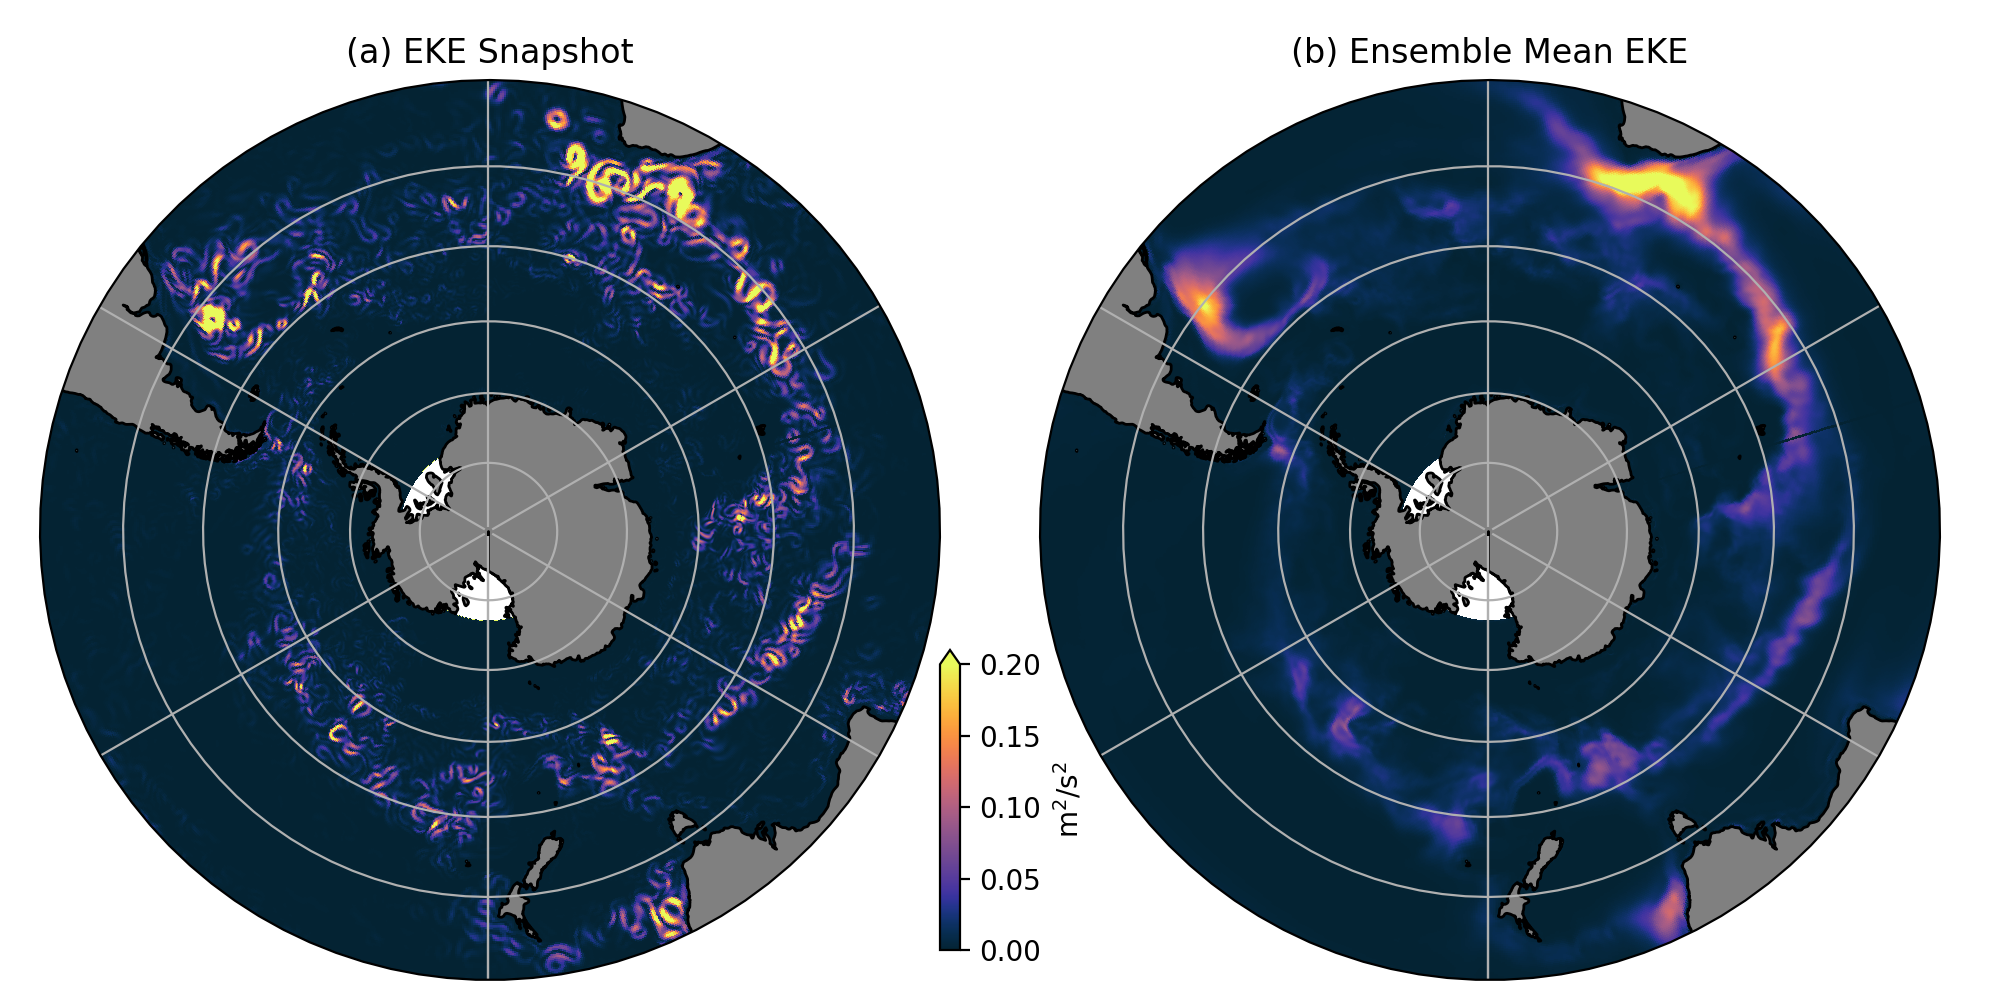
\includegraphics[width=\hsize]{Figure1}
\caption{(a) EKE snapshot and (b) ensemble mean EKE  }
\label{Fig:1}
\end{center}
\end{figure}

For each of the 50 members of the OCCIPUT ensemble we take the EKE averaged over the entire Southern Ocean, and plot the timeseries of this quantity in thin grey lines in Fig.~\ref{Fig:2}(a). 
This plot highlights the considerable spread in EKE, even when averaged over the full circumpolar belt; in other words, there is a significant component of intrinsic variability in the Southern Ocean eddy field.
Nonetheless, when averaged over all ensemble members (red line in Fig.~\ref{Fig:2}a) the coherent, forced, component of eddy variability is revealed.
Averaged over this region the fraction, $R_i$, of intrinsic variance is 0.69, confirming the visual impression that intrinsic processes are dominant here.

\begin{figure}[t]
\begin{center}
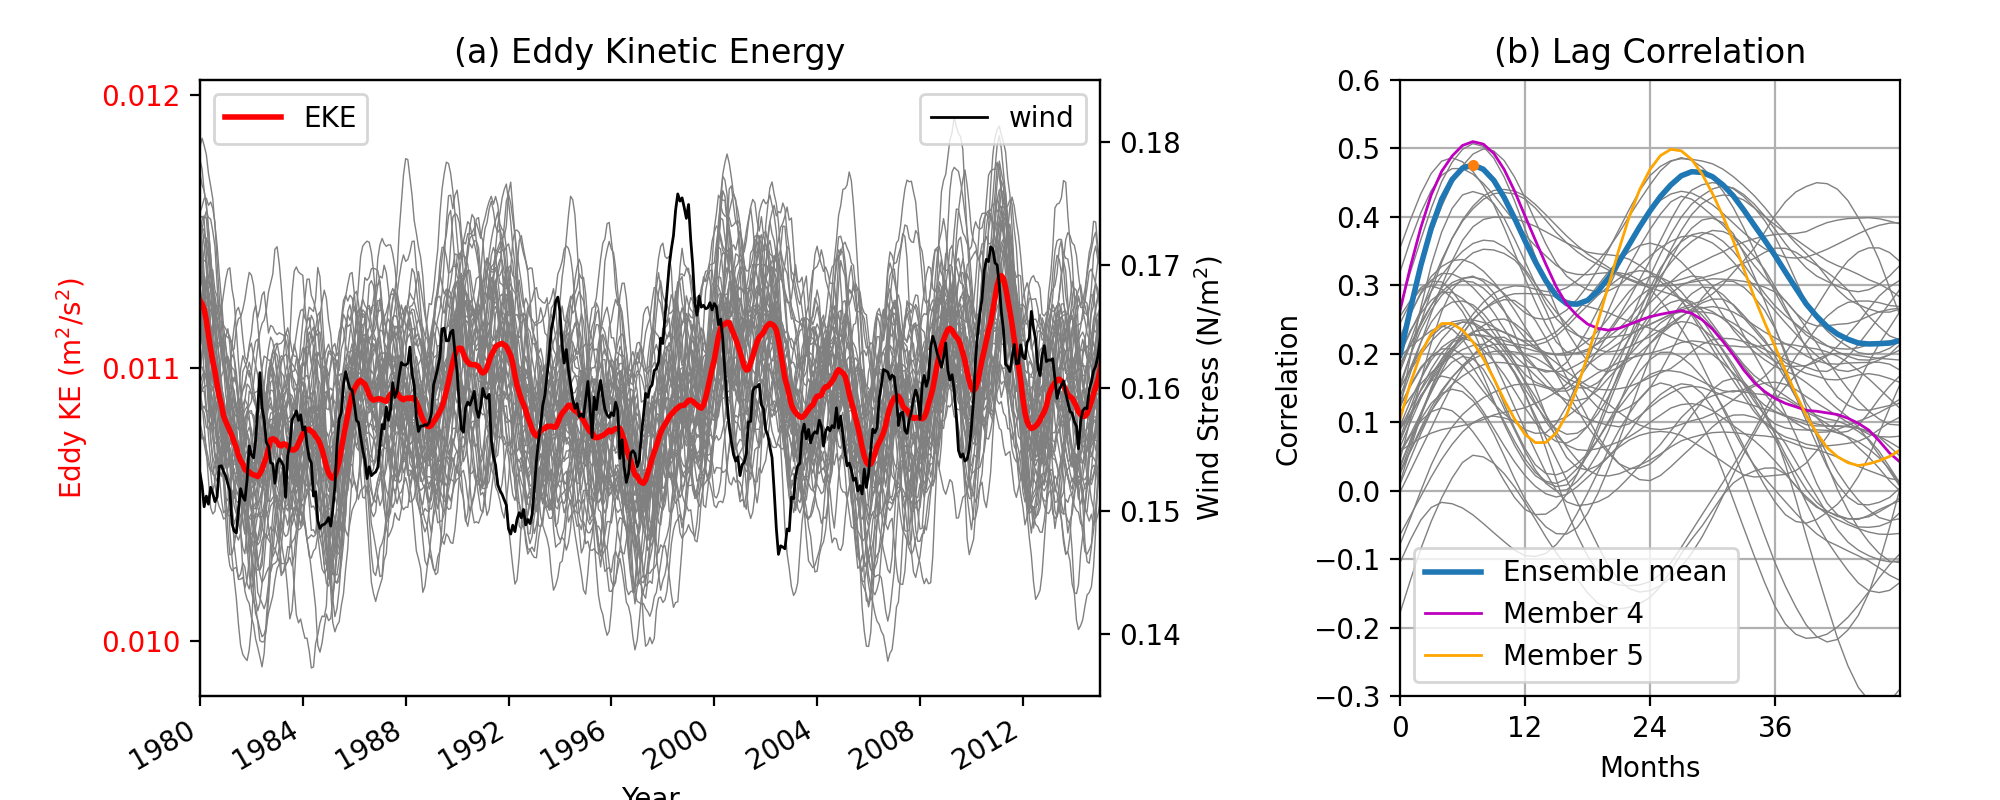
\includegraphics[width=\hsize]{Figure2}
\caption{Eddy kinetic energy statistics over the Southern Ocean (40$^\circ$S--60$^\circ$S). (a) Spatially averaged EKE for individual ensemble members (grey) and the ensemble mean (red) along with wind stress (black); and (b) Time-lagged correlation for the ensemble mean (blue) and individual ensemble  members (grey) -- with two individual ensemble members highlighted in magenta/orange.}
\label{Fig:2}
\end{center}
\end{figure}

Although Southern Ocean EKE is strongly intrinsic, there remains a significant component of forced variability.
Previous studies have suggested that there is a strong contribution of wind stress forcing upon EKE, and we therefore compare the forced variability with the variations in wind stress averaged over the same circumpolar belt (black line in Fig.~\ref{Fig:2}a).
This comparison suggests a relationship in which wind stress leads variations in EKE, consistent with previously published results.
However, the time-lagged correlations between wind stress and EKE suggests that this relationship is complex. 
The intrinsically variable nature of Southern Ocean eddies means that for some ensemble members, there is no meaningful correlation between wind stress and eddies (grey lines in Fig~\ref{Fig:2}b).
On the other hand, ensemble member 4 (magenta line) has a clear an significant (??) correlation with a 7-month lag, while member 5 (orange line) is correlated weakly at 6 months, and strongly correlated at a 28-month lag.
These isolated examples highlight how each ensemble member behaves differently, but the ensemble mean (blue line) includes a correlation at $\sim$6 months and a second clear peak at $\sim$30 months.
Thus, there appear to be two distinct timescales of response of the Southern Ocean eddy field to wind stress. 


\begin{figure}[t]
\begin{center}
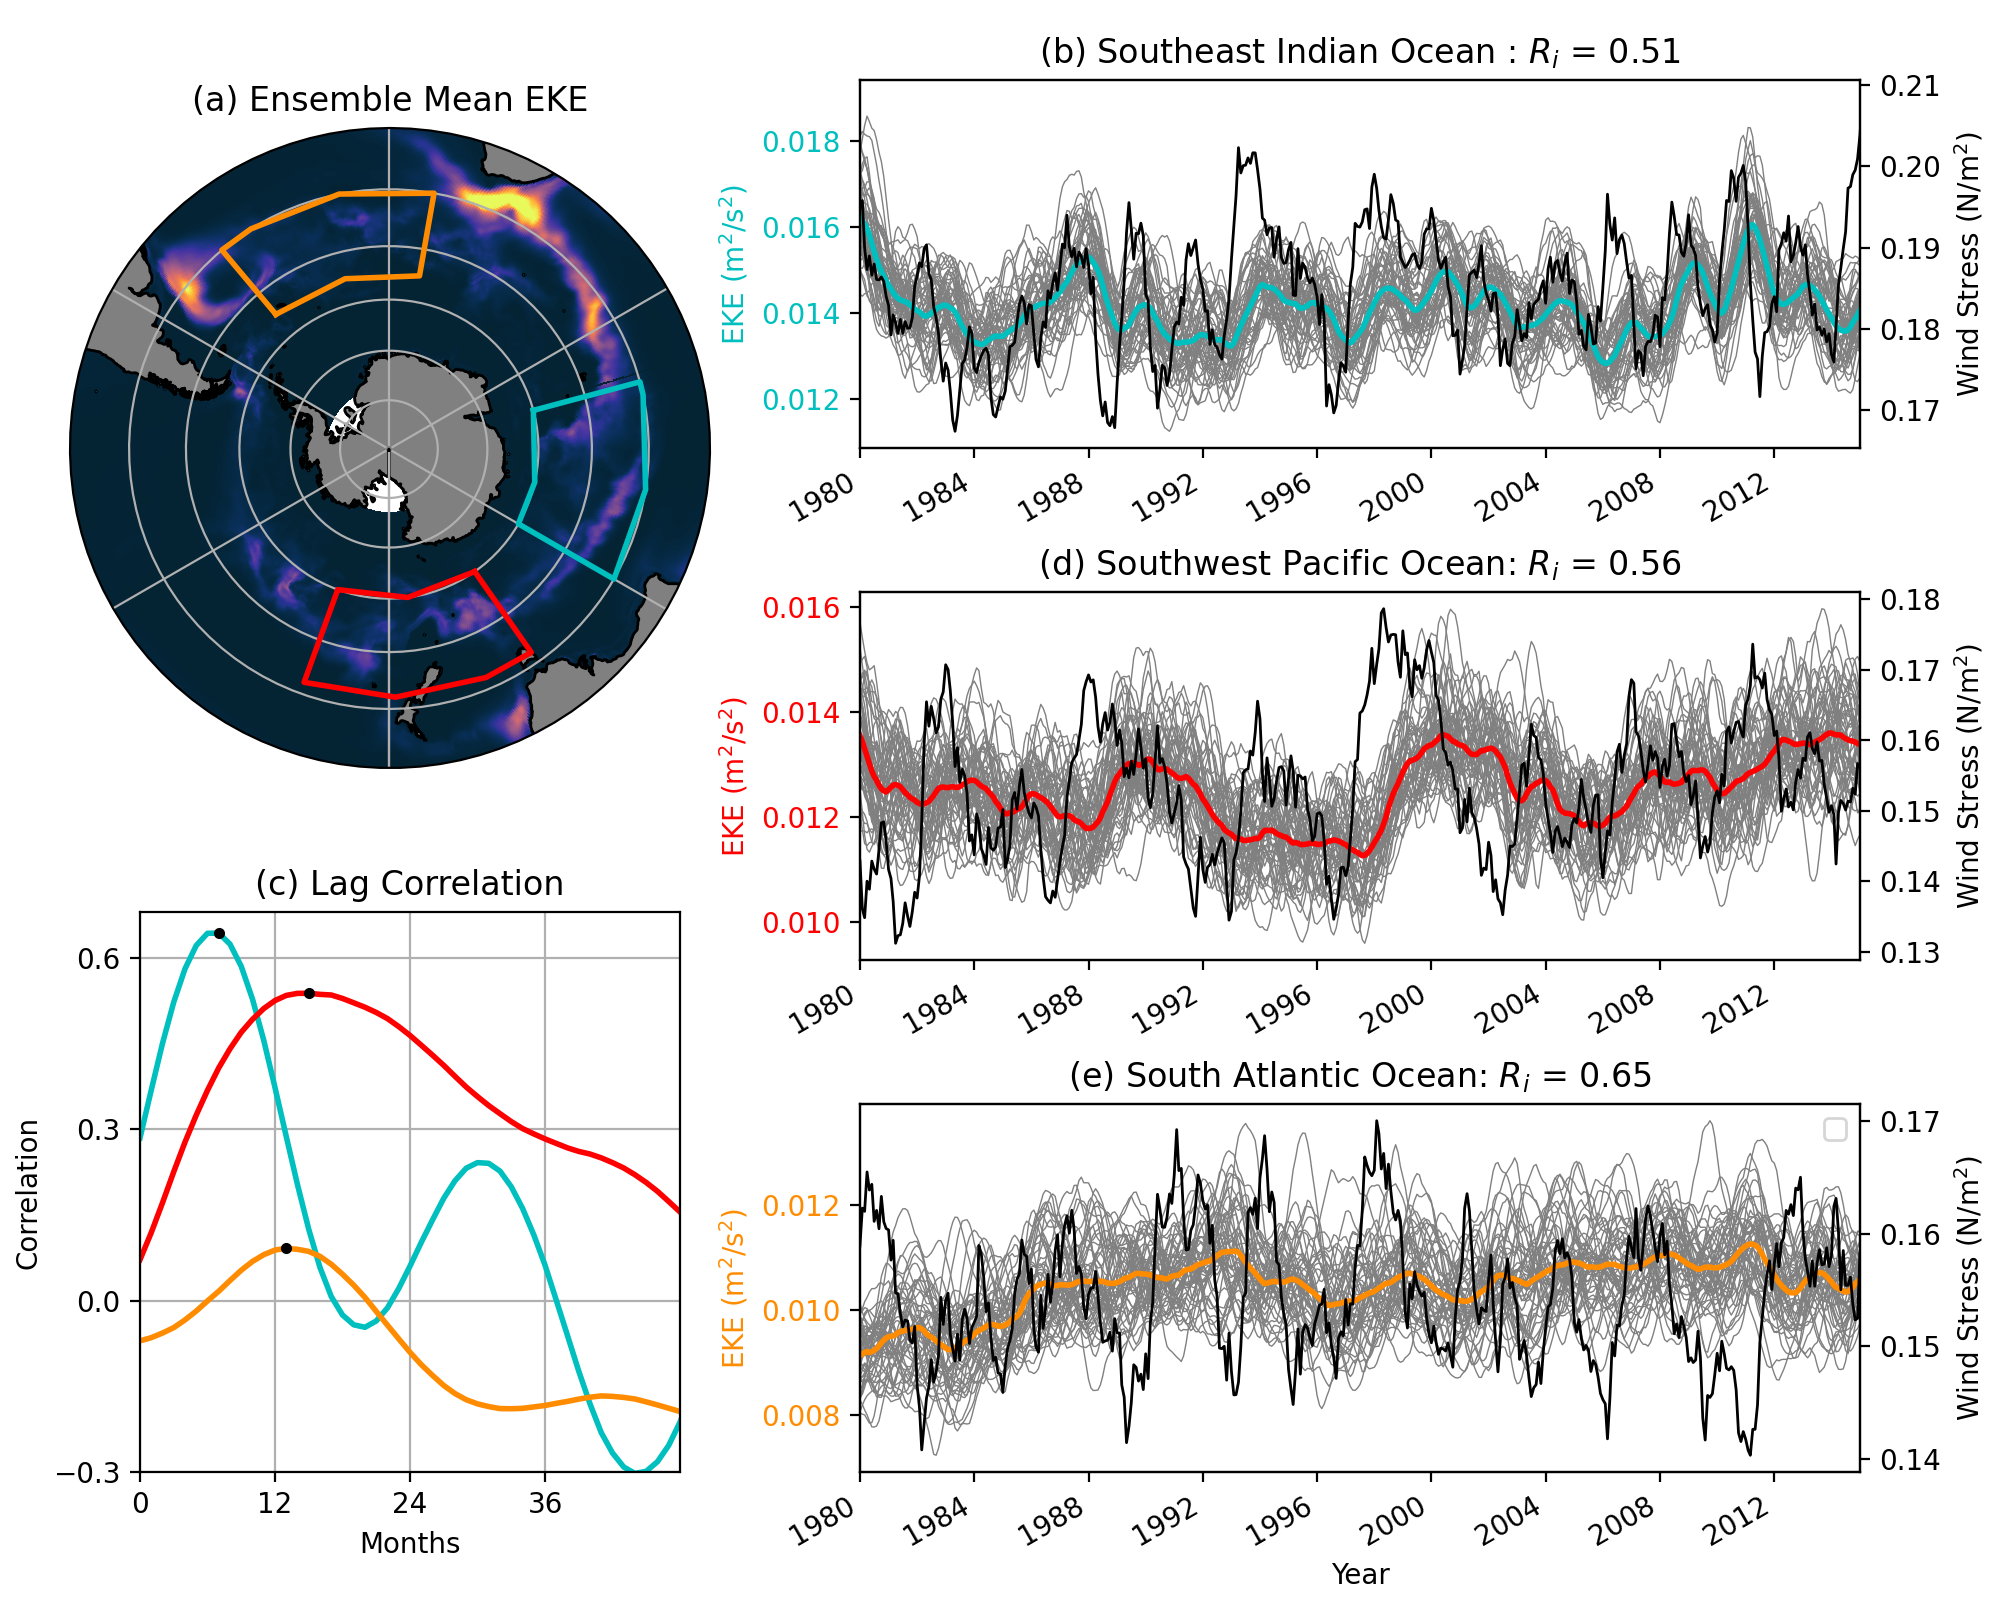
\includegraphics[width=\hsize]{Figure3}
\caption{Eddy kinetic energy statistics within sub-regions of the Southern Ocean. (a) Map showing Ensemble Mean EKE, along with 3 boxes over which a regional EKE analysis is applied; (b) Regional analysis of the Southeast Indian Ocean showing ensemble mean EKE in cyan, individual ensemble members EKE in grey and local wind stress averaged over the region in black; (c) Lagged correlation of ensemble mean EKE in each of the three regions; (d) Regional analysis of the Southwest Pacific Ocean showing ensemble mean EKE in red, individual ensemble members EKE in grey and local wind stress averaged over the region in black; and (3) Regional analysis of the South Atlantic Ocean showing ensemble mean EKE in orange, individual ensemble members EKE in grey and local wind stress averaged over the region in black. The fraction of intrinsic variance in each region is shown in the caption of panels (b), (d) and (e).}
\label{Fig:3}
\end{center}
\end{figure}

The ensemble of simulations shown here allow us to look in more detail at smaller regions of the Southern Ocean.
Calculating the variability of EKE in a smaller region has the advantage of isolating different processes which may occur in differing regions (for example, stronger topographic steering in places with steep bathymetry).
However, this advantage is partly offset by higher intrinsic variability in cases where the region of interest is so small that an individual eddy or event can have a large influence over the EKE timeseries.
In balancing these competing issues, we look at the variability within regions that span 15-20$\circ$ in latitude and 30-40$^\circ$ in longitude, as shown in Figure \ref{Fig:3}(a).
We analyse the EKE timeseries averaged over these boxes -- including individual member EKE, ensemble mean EKE and lagged correlations between local wind stress forcing and the ensemble mean EKE in Fig. \ref{Fig:3}(b-e).

We first examine a region in the lee of Kerguelen Plateau in the Southeast Indian Ocean (cyan box in Fig.~\ref{Fig:3}a).
This region is characterised by high-frequency ($\sim$1 year) variations in EKE, with a relatively large forced component (the intrinsic variance fraction $R_i = 0.51$ which is smaller than the Southern Ocean average; Fig.~\ref{Fig:3}b).
The forced variation is clearly evident in the timeseries of from individual ensemble members; and this forced component is closely related to wind stress.
The lag between wind stress variations and ensemble mean EKE is short ($\sim$ 6 months; Fig.~\ref{Fig:3}c) with a single peak in the lagged correlation.
This region highlights a regime in which the eddy field responds rapidly to variations in the local wind stress.

In the Southeast Pacific Ocean (red box in Fig.~\ref{Fig:3}a) the situation is clearly different.
Here, the intrinsic variance fraction is similar to the Southeast Indian Ocean ($R_i=0.56$) but the timescale of the variability is much longer and there is no significant response to wind stress variations which occur at sub-annual scales (Fig.~\ref{Fig:3}d).
The peak in the lag correlation occurs at approximately 14 months in this region, and again has only a single clear peak.
Thus, this region varies slowly and consistently to multi-year variations in wind stress.

in the South Atlantic Ocean (orange box in Fig.~\ref{Fig:3}a) the system is more dominated by intrinsic variance ($R_i=0.65$) and is poorly correlated with wind stress forcing (Fig.~\ref{Fig:3c,e), reinforcing the circumpolar variability of the EKE response to wind.



Figure 5 -- showing that it is local wind forcing that matters

Figure 6 - Ri ratio plot, and other global features

\section{Discussion}
How do we interpret intrinsic variance ratio in this case?

What can we infer about real world?

Propose hypotheses for two timescales (do we need to test these at all?)



\section{Conclusions}
\begin{itemize}
    \item Intrinsic variance is large.
    \item  Forced component exists and has two timescales.
    \item Short timescale is local eddy response - mixed  barotropic/baroclinic?
    \item Long timescale requires topographic feedback.

\end{itemize}



\acknowledgments
We acknowledge NCI for everything they do for us.

\bibliography{basic_references}

\end{document}